\section{Pipelined MapReduce}
\label{sec:pipelining}
%\begin{figure}[t]
%  \centering
%        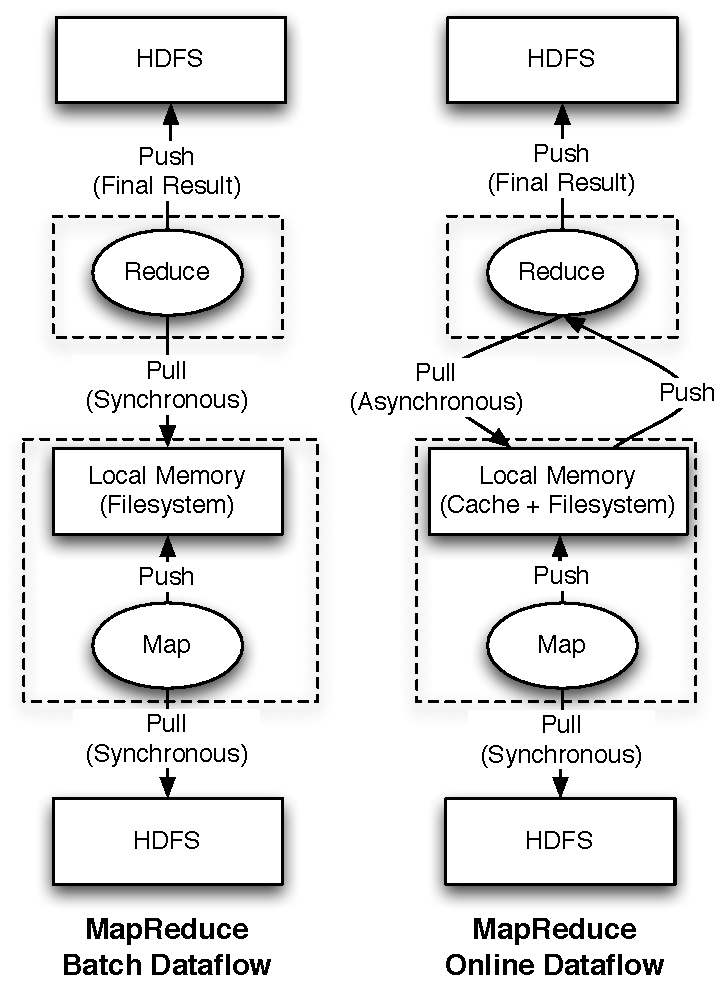
\includegraphics[width=0.90\linewidth]{figures/dataflow_arch.pdf}
%       \caption{Hadoop dataflow for batch (left) and pipelined (right) processing of MapReduce computations.}
%        \label{fig:pipeline}
%\end{figure}

In this section we discuss our extensions to Hadoop to support pipelining
between tasks (Section~\ref{sec:intra-pipe}) and between jobs
(Section~\ref{sec:inter-pipe}).  We describe how our design supports fault
tolerance (Section~\ref{sec:ft}), and discuss the interaction between pipelining
and task scheduling (Section~\ref{sec:pipeline-sched}).  Our focus here is on
batch-processing workloads; we discuss online aggregation and continuous queries
in Section~\ref{sec:online} and Section~\ref{sec:continuous}. We defer
performance results to Section~\ref{sec:perf}.

%Figure~\ref{fig:pipeline} depicts the dataflow of two MapReduce
%implementations. The dataflow on the left corresponds to the output
%materialization approach used by regular Hadoop; the dataflow on the right
%allows pipelining. In the remainder of this section, we present our design and
%implementation for the pipelined Hadoop dataflow. We describe how our design
%supports fault tolerance (Section~\ref{sec:ft}), and discuss the interaction
%between pipelining and task scheduling (Section~\ref{sec:pipeline-sched}).

\subsection{Pipelining Within A Job}
\label{sec:intra-pipe}
As described in Section~\ref{sec:reducetask}, reduce tasks
traditionally issue HTTP requests to \emph{pull} their output from
each {\TT}. This means that map task execution is completely decoupled
from reduce task execution. To support pipelining, we modified the map
task to instead \emph{push} data to reducers as it is produced. To
give an intuition for how this works, we begin by describing a
straightforward pipelining design, and then discuss the changes we
had to make to achieve good performance.

\subsubsection{Na\"{\i}ve Pipelining}
\label{sec:naive}
In our na\"{\i}ve implementation, we modified Hadoop to send data directly from
map to reduce tasks. When a client submits a new job to Hadoop, the {\JT}
assigns the map and reduce tasks associated with the job to the available {\TT}
slots. For purposes of discussion, we assume that there are enough free slots to
assign all the tasks for each job. We modified Hadoop so that each reduce task
contacts every map task upon initiation of the job, and opens a TCP socket which
will be used to pipeline the output of the map function. As each map output
record is produced, the mapper determines which partition (reduce task) the
record should be sent to, and immediately sends it via the appropriate socket.

A reduce task accepts the pipelined data it receives from each map task and
stores it in an in-memory buffer, spilling sorted runs of the buffer to disk as
needed. Once the reduce task learns that every map task has completed, it
performs a final merge of all the sorted runs and applies the user-defined
reduce function as normal.

\subsubsection{Refinements}
\label{sec:pipe-refine}
While the algorithm described above is straightforward, it suffers
from several practical problems. First, it is possible that there will
not be enough slots available to schedule every task in a new
job. Opening a socket between every map and reduce task also requires
a large number of TCP connections. A simple tweak to the na\"{\i}ve
design solves both problems: if a reduce task has not yet been
scheduled, any map tasks that produce records for that partition
simply write them to disk. Once the reduce task is assigned a slot, it
can then pull the records from the map task, as in regular Hadoop.  To
reduce the number of concurrent TCP connections, each reducer can be
configured to pipeline data from a bounded number of mappers at once; the
reducer will pull data from the remaining map tasks in the traditional
Hadoop manner.

% nrc: Not interesting?
Our initial pipelining implementation suffered from a second problem: the map
function was invoked by the same thread that wrote output records to the
pipeline sockets. This meant that if a network I/O operation blocked (e.g.,
because the reducer was over-utilized), the mapper was prevented from doing
useful work. Pipeline stalls should not prevent a map task from making
progress---especially since, once a task has completed, it frees a {\TT} slot
to be used for other purposes. We solved this problem by running the map
function in a separate thread that stores its output in an in-memory buffer, and
then having another thread periodically send the contents of the buffer to the
connected reducers.

\subsubsection{Granularity of Map Output}
\label{sec:mapout}

Another problem with the na\"{\i}ve design is that it eagerly sends
each record as soon as it is produced, which prevents the use of
map-side combiners. Imagine a job where the reduce key has few
distinct values (e.g., gender), and the reduce applies an aggregate
function (e.g., count). As discussed in Section~\ref{sec:progmodel},
combiners allow map-side ``pre-aggregation'': by applying a
reduce-like function to each distinct key at the mapper, network
traffic can often be substantially reduced. Eagerly pipelining each
record as it is produced prevents the use of map-side combiners.

A related problem is that eager pipelining moves some of the sorting
work from the mapper to the reducer. Recall that in the blocking
architecture, map tasks generate sorted spill files: all the reduce
task must do is merge together the pre-sorted map output for each
partition. In the na\"{\i}ve pipelining design, map tasks send output
records in the order in which they are generated, so the reducer must
perform a full external sort. Because the number of map tasks
typically far exceeds the number of reduces~\cite{mapreduce-osdi},
moving more work to the reducer increased response time in our
experiments.

We addressed these issues by modifying the in-memory buffer design described in
Section~\ref{sec:pipe-refine}. Instead of sending the buffer contents to
reducers directly, we wait for the buffer to grow to a threshold
size. The mapper then applies the combiner function, sorts the output by
partition and reduce key, and writes the buffer to disk using the spill file
format described in Section~\ref{sec:maptask}.

Next, we arranged for the {\TT} at each node to handle pipelining data to reduce
tasks. Map tasks register spill files with the {\TT} via RPCs. If the reducers
are able to keep up with the production of map outputs and the network is not a
bottleneck, a spill file will be sent to a reducer soon after it has been
produced (in which case, the spill file is likely still resident in the map
machine's kernel buffer cache). However, if a reducer begins to fall behind, the
number of unsent spill files will grow.

When a map task generates a new spill file, it first queries the {\TT} for the
number of unsent spill files. If this number grows beyond a certain threshold
(two unsent spill files in our experiments), the map task does not immediately
register the new spill file with the {\TT}. Instead, the mapper will accumulate
multiple spill files. Once the queue of unsent spill files falls below the
threshold, the map task merges and combines the accumulated spill files into a
single file, and then resumes registering its output with the {\TT}. This simple
flow control mechanism has the effect of \emph{adaptively} moving load from the
reducer to the mapper or vice versa, depending on which node is the current
bottleneck.

A similar mechanism is also used to control how aggressively the combiner
function is applied. The map task records the ratio between the input and output
data sizes whenever it invokes the combiner function. If the combiner is
effective at reducing data volumes, the map task accumulates more spill files
(and applies the combiner function to all of them) before registering that
output with the {\TT} for pipelining.\footnote{Our current prototype uses a
  simple heuristic: if the combiner reduces data volume by $\frac{1}{k}$ on
  average, we wait until $k$ spill files have accumulated before registering
  them with the {\TT}. A better heuristic would also account for the computational
  cost of applying the combiner function.}

The connection between pipelining and adaptive query processing techniques has
been observed elsewhere (e.g.,~\cite{eddies}). The adaptive scheme outlined
above is relatively simple, but we believe that adapting to feedback along
pipelines has the potential to significantly improve the utilization of
MapReduce clusters.

\subsection{Pipelining Between Jobs}
\label{sec:inter-pipe}

Many practical computations cannot be expressed as a single MapReduce job, and
the outputs of higher-level languages like Pig~\cite{pig} typically involve
multiple jobs.  In the traditional Hadoop architecture, the output of each job
is written to HDFS in the reduce step and then immediately read back from HDFS
by the map step of the next job. Furthermore, the {\JT} cannot schedule a
consumer job until the producer job has completed, because scheduling a map task
requires knowing the HDFS block locations of the map's input split.

In our modified version of Hadoop, the reduce tasks of one job can optionally
pipeline their output directly to the map tasks of the next job, sidestepping
the need for expensive fault-tolerant storage in HDFS for what amounts to a
temporary file. Unfortunately, the computation of the reduce function from the
previous job and the map function of the next job cannot be overlapped: the
final result of the reduce step cannot be produced until all map tasks have
completed, which prevents effective pipelining. However, in the next sections we
describe how online aggregation and continuous query pipelines can publish
``snapshot'' outputs that can indeed pipeline between jobs.

\subsection{Fault Tolerance}
\label{sec:ft}

% nrc: (1) Quantify the overhead added by tracking map task origin (2)
% Did we implement the "don't rerun map task from scratch" idea?

Our pipelined Hadoop implementation is robust to the failure of both
map and reduce tasks. To recover from map task failures, we added
bookkeeping to the reduce task to record which map task produced each
pipelined spill file. To simplify fault tolerance, the reducer treats
the output of a pipelined map task as ``tentative'' until the {\JT}
informs the reducer that the map task has committed successfully. The
reducer can merge together spill files generated by the same
uncommitted mapper, but will not combine those spill files with the
output of other map tasks until it has been notified that the map task
has committed. Thus, if a map task fails, each reduce task can ignore
any tentative spill files produced by the failed map attempt. The
{\JT} will take care of scheduling a new map task attempt, as in stock
Hadoop. 

If a reduce task fails and a new copy of the task is started, the new
reduce instance must be sent all the input data that was sent to the
failed reduce attempt. If map tasks operated in a purely pipelined
fashion and discarded their output after sending it to a reducer, this
would be difficult. Therefore, map tasks retain their output data on
the local disk for the complete job duration. This allows the map's output to be 
reproduced if any reduce tasks fail. For batch jobs, the key advantage of our architecture is
that reducers are not blocked waiting for the complete output of the
task to be written to disk.

Our technique for recovering from map task failure is straightforward, but
places a minor limit on the reducer's ability to merge spill files. To avoid
this, we envision introducing a ``checkpoint'' concept: as a map task runs, it
will periodically notify the {\JT} that it has reached offset $x$ in its input
split. The {\JT} will notify any connected reducers; map task output that was
produced before offset $x$ can then be merged by reducers with other map task
output as normal. To avoid duplicate results, if the map task fails, the new map
task attempt resumes reading its input at offset $x$. This technique would also
reduce the amount of redundant work done after a map task failure or during
speculative execution of ``backup'' tasks~\cite{mapreduce-osdi}.

\subsection{Task Scheduling}
\label{sec:pipeline-sched}

The Hadoop {\JT} had to be retrofitted to support pipelining between jobs. In
regular Hadoop, job are submitted one at a time; a job that consumes the output
of one or more other jobs cannot be submitted until the producer jobs have
completed. To address this, we modified the Hadoop job submission interface to
accept a list of jobs, where each job in the list depends on the job before
it. The client interface traverses this list, annotating each job with the
identifier of the job that it depends on. The {\JT} looks for this annotation
and co-schedules jobs with their dependencies, giving slot preference to
``upstream'' jobs over the ``downstream'' jobs they feed.  As we note in
Section~\ref{sec:concl}, there are many interesting options for scheduling
pipelines or even DAGs of such jobs that we plan to investigate in future.
